
Let,
\begin{align}
    \vec{A} = \myvec{3 \\ 0},
    \vec{B} = \myvec{-2 \\ -2}, 
    \vec{C} = \myvec{8 \\ 2}
\end{align}
Then, 
% Now,
% \begin{align}
% \vec{B - A} = \myvec{-2-3 \\ -2-0}
% = \myvec{-5 \\ -2}
% \end{align}
%
% \begin{align}
% \vec{C - A} = \myvec{8-3 \\ 2-0}
% = \myvec{5 \\ 2}
% \end{align}\\
%
% Forming the matrix $\vec{M}$,
\begin{align}
\vec{M} &= \myvec{\vec{B}-\vec{A}  &  \vec{B}-\vec{C}}^\top \\
        &= \myvec{-5 & 5 \\ -2 & 2}^\top\\
        &= \myvec{-5 & -2 \\ 5 & 2}
\end{align}

Using matrix transformation,
\begin{align}
\vec{M} = \myvec{-5 & -2 \\ 5 & 2} \xleftrightarrow{\text{$R_1$}\rightarrow{\text{$-R_1$}}} 
\myvec{ 5 & 2 \\ 5 & 2} \\
\xleftrightarrow{\text{$R_2$}\rightarrow{\text{$R_2 - R_1$}}}
\myvec{5 & 2 \\ 0 & 0}
\end{align}

$\implies \text{rank}(\vec{M}) = 1$.  Thus, the given points are collinear, as can be verified from Fig. \ref{aug/2/8/Plot}.
 
\begin{figure}[!ht]
\centering
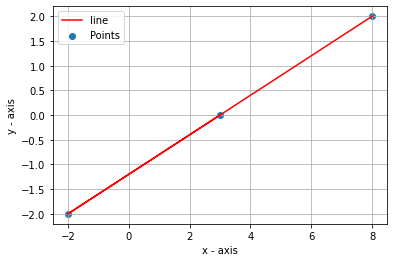
\includegraphics[width=\columnwidth]{solutions/aug/2/8/Figures/Grid.png}
\caption{Plot of the points}
\label{aug/2/8/Plot}
\end{figure}




